%%%%%%%%%%%%%%%%%%%%%%%%%%%%%%%%%%%%%%%%%
% Lachaise Assignment
% LaTeX Template
% Version 1.0 (26/6/2018)
%
% This template originates from:
% http://www.LaTeXTemplates.com
%
% Authors:
% Marion Lachaise & François Févotte
% Vel (vel@LaTeXTemplates.com)
%
% License:
% CC BY-NC-SA 3.0 (http://creativecommons.org/licenses/by-nc-sa/3.0/)
% 
%%%%%%%%%%%%%%%%%%%%%%%%%%%%%%%%%%%%%%%%%

%----------------------------------------------------------------------------------------
%	PACKAGES AND OTHER DOCUMENT CONFIGURATIONS
%----------------------------------------------------------------------------------------

\documentclass{article}

%%%%%%%%%%%%%%%%%%%%%%%%%%%%%%%%%%%%%%%%%
% Lachaise Assignment
% Structure Specification File
% Version 1.0 (26/6/2018)
%
% This template originates from:
% http://www.LaTeXTemplates.com
%
% Authors:
% Marion Lachaise & François Févotte
% Vel (vel@LaTeXTemplates.com)
%
% License:
% CC BY-NC-SA 3.0 (http://creativecommons.org/licenses/by-nc-sa/3.0/)
% 
%%%%%%%%%%%%%%%%%%%%%%%%%%%%%%%%%%%%%%%%%

%----------------------------------------------------------------------------------------
%	PACKAGES AND OTHER DOCUMENT CONFIGURATIONS
%----------------------------------------------------------------------------------------

\usepackage{amsmath,amsfonts,stmaryrd,amssymb} % Math packages

\usepackage[ddmmyyyy]{datetime}
\usepackage{enumerate} % Custom item numbers for enumerations

\usepackage[ruled]{algorithm2e} % Algorithms

\usepackage[framemethod=tikz]{mdframed} % Allows defining custom boxed/framed environments

\usepackage{listings} % File listings, with syntax highlighting
\lstset{
	basicstyle=\ttfamily, % Typeset listings in monospace font
}

%----------------------------------------------------------------------------------------
%	DOCUMENT MARGINS
%----------------------------------------------------------------------------------------

\usepackage{geometry} % Required for adjusting page dimensions and margins

\geometry{
	paper=a4paper, % Paper size, change to letterpaper for US letter size
	top=2.5cm, % Top margin
	bottom=3cm, % Bottom margin
	left=2.5cm, % Left margin
	right=2.5cm, % Right margin
	headheight=14pt, % Header height
	footskip=1.5cm, % Space from the bottom margin to the baseline of the footer
	headsep=1.2cm, % Space from the top margin to the baseline of the header
	%showframe, % Uncomment to show how the type block is set on the page
}

%----------------------------------------------------------------------------------------
%	FONTS
%----------------------------------------------------------------------------------------

\usepackage[utf8]{inputenc} % Required for inputting international characters
\usepackage[T1]{fontenc} % Output font encoding for international characters

\usepackage{XCharter} % Use the XCharter fonts

%----------------------------------------------------------------------------------------
%	COMMAND LINE ENVIRONMENT
%----------------------------------------------------------------------------------------

% Usage:
% \begin{commandline}
%	\begin{verbatim}
%		$ ls
%		
%		Applications	Desktop	...
%	\end{verbatim}
% \end{commandline}

\mdfdefinestyle{commandline}{
	leftmargin=10pt,
	rightmargin=10pt,
	innerleftmargin=15pt,
	middlelinecolor=black!50!white,
	middlelinewidth=2pt,
	frametitlerule=false,
	backgroundcolor=black!5!white,
	frametitle={Command Line},
	frametitlefont={\normalfont\sffamily\color{white}\hspace{-1em}},
	frametitlebackgroundcolor=black!50!white,
	nobreak,
}

% Define a custom environment for command-line snapshots
\newenvironment{commandline}{
	\medskip
	\begin{mdframed}[style=commandline]
}{
	\end{mdframed}
	\medskip
}

%----------------------------------------------------------------------------------------
%	FILE CONTENTS ENVIRONMENT
%----------------------------------------------------------------------------------------

% Usage:
% \begin{file}[optional filename, defaults to "File"]
%	File contents, for example, with a listings environment
% \end{file}

\mdfdefinestyle{file}{
	innertopmargin=1.6\baselineskip,
	innerbottommargin=0.8\baselineskip,
	topline=false, bottomline=false,
	leftline=false, rightline=false,
	leftmargin=2cm,
	rightmargin=2cm,
	singleextra={%
		\draw[fill=black!10!white](P)++(0,-1.2em)rectangle(P-|O);
		\node[anchor=north west]
		at(P-|O){\ttfamily\mdfilename};
		%
		\def\l{3em}
		\draw(O-|P)++(-\l,0)--++(\l,\l)--(P)--(P-|O)--(O)--cycle;
		\draw(O-|P)++(-\l,0)--++(0,\l)--++(\l,0);
	},
	nobreak,
}

% Define a custom environment for file contents
\newenvironment{file}[1][File]{ % Set the default filename to "File"
	\medskip
	\newcommand{\mdfilename}{#1}
	\begin{mdframed}[style=file]
}{
	\end{mdframed}
	\medskip
}

%----------------------------------------------------------------------------------------
%	NUMBERED QUESTIONS ENVIRONMENT
%----------------------------------------------------------------------------------------

% Usage:
% \begin{question}[optional title]
%	Question contents
% \end{question}

\mdfdefinestyle{question}{
	innertopmargin=1.2\baselineskip,
	innerbottommargin=0.8\baselineskip,
	roundcorner=5pt,
	nobreak,
	singleextra={%
		\draw(P-|O)node[xshift=1em,anchor=west,fill=white,draw,rounded corners=5pt]{%
		Question \theQuestion\questionTitle};
	},
}

\newcounter{Question} % Stores the current question number that gets iterated with each new question

% Define a custom environment for numbered questions
\newenvironment{question}[1][\unskip]{
	\bigskip
	\stepcounter{Question}
	\newcommand{\questionTitle}{~#1}
	\begin{mdframed}[style=question]
}{
	\end{mdframed}
	\medskip
}

%----------------------------------------------------------------------------------------
%	WARNING TEXT ENVIRONMENT
%----------------------------------------------------------------------------------------

% Usage:
% \begin{warn}[optional title, defaults to "Warning:"]
%	Contents
% \end{warn}

\mdfdefinestyle{warning}{
	topline=false, bottomline=false,
	leftline=false, rightline=false,
	nobreak,
	singleextra={%
		\draw(P-|O)++(-0.5em,0)node(tmp1){};
		\draw(P-|O)++(0.5em,0)node(tmp2){};
		\fill[black,rotate around={45:(P-|O)}](tmp1)rectangle(tmp2);
		\node at(P-|O){\color{white}\scriptsize\bf !};
		\draw[very thick](P-|O)++(0,-1em)--(O);%--(O-|P);
	}
}

% Define a custom environment for warning text
\newenvironment{warn}[1][Warning:]{ % Set the default warning to "Warning:"
	\medskip
	\begin{mdframed}[style=warning]
		\noindent{\textbf{#1}}
}{
	\end{mdframed}
}

%----------------------------------------------------------------------------------------
%	INFORMATION ENVIRONMENT
%----------------------------------------------------------------------------------------

% Usage:
% \begin{info}[optional title, defaults to "Info:"]
% 	contents
% 	\end{info}

\mdfdefinestyle{info}{%
	topline=false, bottomline=false,
	leftline=false, rightline=false,
	nobreak,
	singleextra={%
		\fill[black](P-|O)circle[radius=0.4em];
		\node at(P-|O){\color{white}\scriptsize\bf i};
		\draw[very thick](P-|O)++(0,-0.8em)--(O);%--(O-|P);
	}
}

% Define a custom environment for information
\newenvironment{info}[1][Info:]{ % Set the default title to "Info:"
	\medskip
	\begin{mdframed}[style=info]
		\noindent{\textbf{#1}}
}{
	\end{mdframed}
}
 % Include the file specifying the document structure and custom commands

%----------------------------------------------------------------------------------------
%	ASSIGNMENT INFORMATION
%----------------------------------------------------------------------------------------

\title{Prova 22/05/2025} % Title of the assignment

\author{Rocco Lo Russo\\ \texttt{roc.lorusso@studenti.unina.it}} % Author name and email address

\date{Università di Napoli Federico II - DIETI --- \today} % University, school and/or department name(s) and a date

%----------------------------------------------------------------------------------------

\begin{document}

\maketitle % Print the title

%----------------------------------------------------------------------------------------
%	INTRODUCTION
%----------------------------------------------------------------------------------------

\section*{Introduzione} % Unnumbered section
In questo documento verrà sviluppata la prova intercorso del 22/05/2025, esponendo analiticamente i seguenti punti: \textbf{mappa della memoria}, \textbf{pseudocodice} e implementazione in \textbf{ASIM}.

% Math equation/formula
% \begin{equation}
% 	I = \int_{a}^{b} f(x) \; \text{d}x.
% \end{equation}

% \begin{info} % Information block

% \end{info}


\section{Traccia} \label{sec:traccia}% Numbered section 

Un sistema è composto da 3 unità, A, B e C, tra loro collegate mediante due periferiche parallele che interconnettono A con B e A con C rispettivamente. I messaggi hanno un primo carattere identificativo che può essere pari a 0 a un valore diverso da 0. Il sistema opera in due fasi successive come descritto di seguito:
\begin{itemize}
	\item Fase 1: A riceve K messaggi di N caratteri da B e da C in modo alternato. In ordine non prefissato, quindi si parte da B o da C, e \textbf{non ci sono sovrapposizioni tra i messaggi ricevuti da B o da C};
	\item Fase 2: Al termine della fase 1, il nodo A continua nella stessa modalità alternata e termina la ricezione dei messaggi se due messaggi ricevuti (dalle due diverse periferiche) hanno il carattere identificativo del messaggio pari a 0.
\end{itemize}

%------------------------------------------------

\subsection{Analisi della traccia}
Dalla traccia emerge che la comunicazione debba essere gestita in modo tale da garantire la \textit{non sovrapposizione} dei messaggi ricevuti da B e da C. Questo implica che verrà utilizzato un unico buffer di ricezione in cui verranno conservati i messaggi ricevuti, e che una periferica non potrà mandare un nuovo carattere se l'altra non avrà finito la trasmissione di un intero messaggio. La ricezione dei messaggi in modo alternato pone il vincolo, nella codifica della ISR, di considerare casuale la provenienza del primo messaggio. Ci sono due modi di interpretare questo passo della traccia:
\begin{itemize}
	\item Il primo messaggio può arrivare da qualsiasi periferica, e una volta arrivato questo stabilisce l'ordine di arrivo di tutti gli altri K-1 messaggi;
	\item I messaggi vengono ricevuti in modo alternato ma a coppie, ovvero \textbf{per ogni coppia} il primo messaggio può provenire da qualsiasi periferica, ma il secondo deve provenire necessariamente dall'altra.
\end{itemize}
La soluzione presentata più avanti si basa sulla seconda interpretazione. Sotto questi vincoli, i conflitti da gestire sono:
\begin{itemize}
	\item Accesso in mutua esclusione in scrittura alla risorsa rappresentata dal nodo A, in modo da garantire la non sovrapposizione dei messaggi;
	\item Regolare l'accesso alla risorsa in modo che sia alternato, curando i casi in cui le ISR pongano una periferica in stato di attesa. 
\end{itemize}

% Numbered question, with subquestions in an enumerate environment
% \begin{question}
% 	Quisque ullamcorper placerat ipsum. Cras nibh. Morbi vel justo vitae lacus tincidunt ultrices. Lorem ipsum dolor sit amet, consectetuer adipiscing elit.

% 	% Subquestions numbered with letters
% 	\begin{enumerate}[(a)]
% 		\item Do this.
% 		\item Do that.
% 		\item Do something else.
% 	\end{enumerate}
% \end{question}
	
%------------------------------------------------

% \begin{center}
% 	\begin{minipage}{0.5\linewidth} % Adjust the minipage width to accomodate for the length of algorithm lines
% 		\begin{algorithm}[H]
% 			\KwIn{$(a, b)$, two floating-point numbers}  % Algorithm inputs
% 			\KwResult{$(c, d)$, such that $a+b = c + d$} % Algorithm outputs/results
% 			\medskip
% 			\If{$\vert b\vert > \vert a\vert$}{
% 				exchange $a$ and $b$ \;
% 			}
% 			$c \leftarrow a + b$ \;
% 			$z \leftarrow c - a$ \;
% 			$d \leftarrow b - z$ \;
% 			{\bf return} $(c,d)$ \;
% 			\caption{\texttt{FastTwoSum}} % Algorithm name
% 			\label{alg:fastTwoSum}   % optional label to refer to
% 		\end{algorithm}
% 	\end{minipage}
% \end{center}

% % Numbered question, with an optional title
% \begin{question}[\itshape (with optional title)]

% \end{question}

\section{Mappa della memoria}
In questa sezione verrà presentata una mappa della memoria del nodo A in accordo a quanto specificato nel file .cfg utilizzato nella simulazione e in accordo alla memoria caricata (\textit{file rom.mem}).

\begin{center}
    
    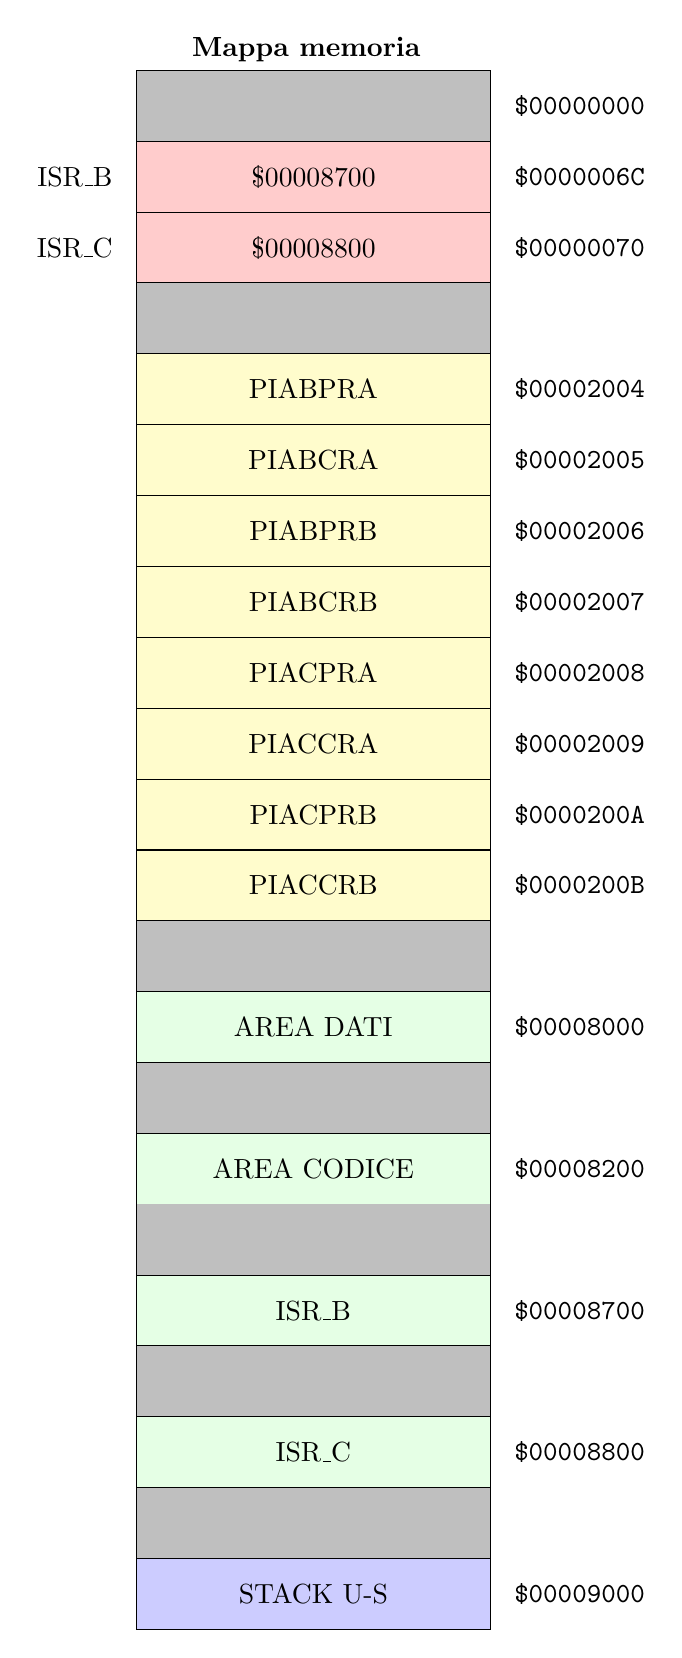
\begin{tikzpicture}[scale=0.9]
        % Rettangolo principale
        \draw (0,0) rectangle (5,20);
        \node at (2.4,20.3) {\textbf{Mappa memoria}};
        
        % vuoto
        \draw (0,20) rectangle (5,19);
        \node[right=5pt] at (5,19.5) {\texttt{\$00000000}};
        \fill[lightgray] (0,20) rectangle (5,19);
        % INT3
        \fill[red!20](0,19) rectangle (5,17);
        \draw (0,19) rectangle (5,18);
        \node[left=5pt] at (0,18.5) {ISR\_B};
        \node[right=5pt] at (5,18.5) {\texttt{\$0000006C}};
        \node at (2.5,18.5) {\$00008700}; 
        
        % INT4 
        \draw (0,18) rectangle (5,17);
        \node[left=5pt] at (0,17.5) {ISR\_C};
        \node[right=5pt] at (5,17.5) {\texttt{\$00000070}};
        \node at (2.5,17.5) {\$00008800};

        % vuoto
        \draw (0,17) rectangle (5,16);
        \fill[lightgray] (0,17) rectangle (5,16);
        %PIA 
        \fill[yellow!20](0,16) rectangle (5,8);
        \draw(0,16) rectangle (5,15);
        \node[right=5pt] at (5,15.5) {\texttt{\$00002004}};
        \node at (2.5,15.5) {PIABPRA};
        \draw(0,15) rectangle (5,14);
        \node[right=5pt] at (5,14.5) {\texttt{\$00002005}};
        \node at (2.5,14.5) {PIABCRA};
        \draw(0,14) rectangle (5,13);
        \node[right=5pt] at (5,13.5) {\texttt{\$00002006}};
        \node at (2.5,13.5) {PIABPRB};
        \draw(0,13) rectangle (5,12);
        \node[right=5pt] at (5,12.5) {\texttt{\$00002007}};
        \node at (2.5,12.5) {PIABCRB};

        \draw(0,12) rectangle (5,11);
        \node[right=5pt] at (5,11.5) {\texttt{\$00002008}};
        \node at (2.5,11.5) {PIACPRA};
        \draw(0,11) rectangle (5,10);
        \node[right=5pt] at (5,10.5) {\texttt{\$00002009}};
        \node at (2.5,10.5) {PIACCRA};
        \draw(0,10) rectangle (5,9);
        \node[right=5pt] at (5,9.5) {\texttt{\$0000200A}};
        \node at (2.5,9.5) {PIACPRB};
        \draw(0,9) rectangle (5,8);
        \node[right=5pt] at (5,8.5) {\texttt{\$0000200B}};
        \node at (2.5,8.5) {PIACCRB};

        % vuoto
        \draw (0,8) rectangle (5,7);
        \fill[lightgray] (0,8) rectangle (5,7);
        
        % DATI
        \fill[green!10] (0,7) rectangle (5,0);
        \draw(0,7) rectangle (5,6);
        \node[right=5pt] at (5,6.5) {\texttt{\$00008000}};
        \node at (2.5,6.5) {AREA DATI};

        
        % vuoto
        \draw (0,6) rectangle (5,5);
        \fill[lightgray] (0,6) rectangle (5,5);
        
        % CODICE
        \draw(0,5) rectangle (5,4);
        \node[right=5pt] at (5,4.5) {\texttt{\$00008200}};
        \node at (2.5,4.5) {AREA CODICE};

        % vuoto
        \draw (0,4) rectangle (5,3);
        \fill[lightgray] (0,4) rectangle (5,3);

        % ISRB 
        \draw(0,3) rectangle (5,2);
        \node[right=5pt] at (5,2.5) {\texttt{\$00008700}};
        \node at (2.5,2.5) {ISR\_B};

        % vuoto
        \draw (0,2) rectangle (5,1);
        \fill[lightgray] (0,2) rectangle (5,1);

        % ISRC
        \draw(0,1) rectangle (5,0);
        \node[right=5pt] at (5,0.5) {\texttt{\$00008800}};
        \node at (2.5,0.5) {ISR\_C};

        % vuoto 
        \draw(0,0) rectangle (5,-1);
        \fill[lightgray](0,0) rectangle (5,-1);
        % STACK
        \fill[blue!20](0,-1) rectangle (5,-2);
        \draw (0,-1) rectangle (5,-2);
        \node[right=5pt] at (5,-1.5) {\texttt{\$00009000}};
        \node at (2.5,-1.5) {STACK U-S};

        \draw(0,-2) rectangle (5,20); % ricalco bordi
    \end{tikzpicture}
\end{center}

% % File contents
% \begin{file}[hello.py]
% \begin{lstlisting}[language=Python]
% #! /usr/bin/python

% import sys
% sys.stdout.write("Hello World!\n")
% \end{lstlisting}
% \end{file}



% % Command-line "screenshot"
% \begin{commandline}
% 	\begin{verbatim}
% 		$ chmod +x hello.py
% 		$ ./hello.py

% 		Hello World!
% 	\end{verbatim}
% \end{commandline}


% Warning text, with a custom title
% \begin{warn}[Osservazione:]

% \end{warn}

%----------------------------------------------------------------------------------------

\section{Implementazione}
In questa sezione verrà presentato il codice assembly per Motorola68000 e lo pseudocodice usato come riferimento per l'implementazione.

\subsection{Variabili}
Descrizione delle variabili utilizzate: 
\\

\begin{description}[style=nextline,leftmargin=3.45cm,labelwidth=2.8cm,labelsep=0.6cm,font=\ttfamily\bfseries]
  \item[fine] Intero che può assumere i valori 0 (il nodo A è in ricezione) o 1 (il nodo A ha terminato la ricezione).
  \item[lock] Intero che può assumere i valori 0 o 1, viene testato dall'istruzione atomica TAS per garantire l'accesso mutualmente esclusivo alla sezione critica.
  \item[possesso] Intero che può assumere i valori -1 (\texttt{is\_free}), 0 (\texttt{is\_reading\_b}) o 1 (\texttt{is\_reading\_c}).
  \item[buff] Puntatore alla prima locazione di un vettore di dimensione K*N di caratteri; serve per accedere alla memoria del nodo A.
  \item[curr] Intero da 0 a N che tiene conto dei caratteri ricevuti.
  \item[tot] Intero da 0 a K*N per l’accesso indirizzato al vettore dei caratteri.
  \item[msg] Intero da 0 a K che conta i messaggi ricevuti.
  \item[end\_b,(end\_c)] Intero: 0 se il messaggio da b (c) non è terminato, 1 altrimenti.
  \item[fase2] Intero: 0 (fase 1), 1 (fase 2).
  \item[cond\_b,(cond\_c)] Intero: 0 se il primo carattere ricevuto da b (c) non è 0, 1 altrimenti.
  \item[b\_sus,(c\_sus)] Intero: 0 se b (c) non è bloccato, 1 se è in attesa che venga letto il carattere.
  \item[idx] Variabile temporanea per memorizzare un valore della variabile \texttt{tot}.
\end{description}
\newpage
\subsection{Pseudocodice}
Assumiamo che ISR\_B e ISR\_C siano speculari, e che ISR\_B sia più prioritaria di ISR\_C : se il nodo A riceve un messaggio da C durante l'esecuzione di ISR\_B, ISR\_C prelaziona ISR\_B. Come anticipato nella sezione \ref{sec:traccia}, l'accesso alla sezione critica in cui si controlla ed eventualmente modifica la variabile \textit{possesso} avverrà in mutua esclusione.

\vspace{2\baselineskip}
\begin{lstlisting}
# define is_reading_b 0
# define is_reading_c 1
# define is_free -1 

void isr_b(){
    if(!fine){
        if(TAS(lock)){
            if(possesso !=c and !end_b){
                possesso = is_reading_b;
            }
            lock = 0;
        }else{
            RTE;
        }

        switch (possesso){
            case is_reading_b:
                buff[tot] = PIABPRA;
                if(curr == 0 && fase2 && buff[tot] == 0){
                    cond_b = 1;
                }
                tot++;
                curr++;
                if(curr == N){
                    curr = 0;
                    msg++;
                    end_b = 1;
                    possesso = is_free;
                    if(end_c){
                        end_b = 0;
                        end_c = 0;
                        if(msg==k){
                            fase2=1;
                        }
                    }
                    if(fase2 && (cond_b && cond_c)){
                        fine = 1;
                    }
                    if(c_sus && !end_c){
                        tot++;
                        curr++;
                        buff[tot-1] = PIACPRA;
                        // se c interrompe qui, trovera' possesso=is_free
                        if(buff[tot-1] == 0 && fase2){
                            cond_c=1;
                        }
                        possesso = is_reading_c;
                    }
                }
             case is_free:
                if(c_sus && !end_c){
                    tot++;
                    curr++;
                    buff[tot-1] = PIACPRA;
                    if(buff[tot-1] == 0 && fase2){
                        cond_c=1;
                    }
                    possesso = is_reading_c;
                }
            case is_reading_c{
                if(c_sus){
                // L'unica assunzione possibile e' che 
                // questo non sia il primo carattere di b
                    idx = tot;
                    tot++;
                    curr++;
                    possesso = is_reading_c;
                    if(curr == N){
                        curr = 0;
                        msg++;
                        end_c = 1;
                        possesso = is_free;
                        if (end_b){
                            end_b = 0;
                            end_c = 0;
                            if(msg == k){
                                fase2=1;
                            }
                        }
                        if(fase2 && (cond_b && cond_c)){
                            fine = 1;
                        }
                        if(!end_b){
                            buff[tot]=PIABPRA;
                            tot++;
                            curr++;
                            if(fase2 && buff[tot-1]==0){
                                cond_b = 1;
                            }
                            possesso = is_reading_b;
                        }
                    }
                    buff[idx]=PIACPRA;
                }
            }
        }   
        RTE;
    }else{  // se fine == 1
        RTE;
    }
} // fine isr_b 
\end{lstlisting}
\newpage
\subsection{Codice assembly MC68000}
Di seguito viene esposta la codifica in assembly, basata sullo pseudocodice esposto nel paragrafo precedente, del programma eseguito dal nodo A e delle ISR relative alla ricezioni di caratteri sulla parallela proveniente da B e C. I programmi eseguiti dai nodi B e C consistono in semplici cicli di invio di messaggi tramite parallela. 
\vspace{2\baselineskip}

\begin{lstlisting}[language=RISCAsm]
        ORG     $8000       * AREA DATI
FINE    DC.B    0
LOCK    DC.B    0
POSS    DC.B    -1
CURR    DC.B    0
TOT     DC.B    0
MSG     DC.B    0 
END_B   DC.B    0 
END_C   DC.B    0 
FASE2   DC.B    0
COND_B  DC.B    0
COND_C  DC.B    0
BUFF    DS.B    18

        ORG     $8200       * AREA CODICE
PIABPRA EQU     $2004
PIABCRA EQU     $2005
PIACPRA EQU     $2008
PIACCRA EQU     $2009
N       EQU     3
K       EQU     6

MAIN    JSR     PIAINIT
        MOVE.W  SR,D0 
        ANDI.W  #$D8FF,D0
        MOVE.W  D0,SR 
LOOP    JMP     LOOP 


PIAINIT MOVE    #$00,PIABCRA 
        MOVE    #$00,PIABPRA 
        MOVE    #%00100101,PIABCRA 
        MOVE    #$00,PIACCRA 
        MOVE    #$00,PIACPRA 
        MOVE    #%00100101,PIACCRA
        RTS  

        ORG     $8700
ISR_B   MOVEM.L D0-D7/A0-A2,-(SP)
        MOVE    FINE,D0 
        CMP     #$01,D0 
        BEQ     RETURN 
        TAS     LOCK 
        BNE     RETURN 
        MOVE    POSS,D0
        CMP     #1,D0 
        BEQ     CONT0
        MOVE    END_B,D0 
        CMP     #1,D0 
        BEQ     CONT0 
        MOVE    #0,POSS 
CONT0   MOVE    #0,LOCK 
        MOVE    POSS,D0
        CMP     #1,D0 
        BEQ     CASE1
        CMP     #-1,D0 
        BEQ     CASE2 
        MOVEA.L #PIABPRA,A0     * is_reading_b  
        MOVEA.L #BUFF,A1 
        MOVE    TOT,D0 
        MOVE    CURR,D1 
        MOVE    (A0),(A1,D0)
        MOVE    (A1,D0),D2 
        MOVE    FASE2,D3 
        CMP     #0,D2
        BNE     CONT1 
        CMP     #1,D3 
        BNE     CONT1 
        CMP     #0,D1 
        BNE     CONT1
        MOVE    #1,COND_B
CONT1   ADDQ    #1,D0
        ADDQ    #1,D1 
        MOVE    D0,TOT 
        MOVE    D1,CURR 
        CMP     #N,D1 
        BNE     RETURN 
        MOVE    #0,CURR 
        MOVE    MSG,D0 
        ADDQ    #1,D0 
        MOVE    D0,MSG 
        MOVE    #1,END_B
        MOVE    #-1,POSS
        MOVE    END_C,D1
        CMP     #1,D1 
        BNE     CONT2 
        MOVE    #0,END_B
        MOVE    #0,END_C 
        CMP     K,D0 
        BNE     CONT2 
        MOVE    #1,FASE2
CONT2   MOVE    FASE2,D0 
        CMP     #1,D0 
        BNE     CONT3 
        MOVE    END_B,D0 
        CMP     #1,D0 
        BNE     CONT3
        MOVE    END_C,D0 
        CMP     #1,D0 
        BNE     CONT3
        MOVE    #1,FINE         * controllo c_sus 
CONT3   MOVE    PIACCRA,D0 
        ANDI    #%10000000,D0 
        BEQ     RETURN 
        MOVE    END_C,D0 
        CMP     #1,D0 
        BNE     RETURN 
        MOVEA.L #PIACPRA,A0 
        MOVEA.L #BUFF,D0
        MOVE    TOT,D0
        MOVE    TOT,D7 
        MOVE    CURR,D1 
        ADDQ    #1,D0
        ADDQ    #1,D1 
        MOVE    D0,TOT 
        MOVE    D1,CURR 
        MOVE    (A1),(A0,D7)
        MOVE    (A0,D7),D0 
        MOVE    FASE2,D1 
        CMP     #1,D1 
        BNE     CONT4
        CMP     #0,D0 
        BNE     CONT4 
        MOVE    #1,COND_C
CONT4   MOVE    #1,POSS 
        JMP     RETURN 
CASE1   MOVE    PIACCRA,D0      * is_reading_c 
        ANDI    #%10000000,D0 
        BEQ     RETURN 
        MOVE    TOT,D7 
        MOVE    TOT,D0 
        MOVE    CURR,D1 
        ADDQ    #1,D0
        ADDQ    #1,D1
        MOVE    D0,TOT
        MOVE    D1,CURR 
        MOVE    #1,POSS 
        CMP     N,D1 
        BNE     CONT5
        MOVE    #0,CURR 
        MOVE    MSG,D0 
        ADDQ    #1,D0  
        MOVE    D0,MSG 
        MOVE    #1,END_C 
        MOVE    #-1,POSS 
        MOVE    END_B,D0 
        CMP     #1,D0 
        BNE     CONT6
        MOVE    #0,END_B
        MOVE    #0,END_C 
        MOVE    MSG,D0 
        CMP     K,D0
        BNE     CONT6
        MOVE    #1,FASE2 
CONT6   MOVE    FASE2,D0 
        CMP     #1,D0 
        BNE     CONT7
        MOVE    COND_B,D0 
        CMP     #1,D0 
        BNE     CONT7 
        MOVE    COND_C,D0 
        CMP     #1,D0 
        BNE     CONT7 
        MOVE    #1,FINE 
CONT7   MOVE    END_B,D0 
        CMP     #1,D0 
        BNE     CONT5 
        MOVE    TOT,D0 
        MOVE    CURR,D1 
        MOVEA.L #PIABDRA,A0
        MOVEA.L #BUFF,A1 
        MOVE    (A0),(A1,D0)
        MOVE    (A1,D0),D2
        ADDQ    #1,D0 
        ADDQ    #1,D1 
        MOVE    D0,TOT 
        MOVE    D1,CURR 
        MOVE    FASE2,D3 
        CMP     #1,D3
        BNE     CONT8 
        CMP     #0,D2 
        BNE     CONT8 
        MOVE    #1,COND_B 
CONT8   MOVE    #0,POSS 
CONT5   MOVEA.L #PIACPRA,A0 
        MOVEA.L #BUFF,A1 
        MOVE    (A0),(A1,D7)
        JMP     RETURN 
CASE2   MOVE    PIACCRA,D0      * is_free 
        ANDI    #%10000000,D0   
        BEQ     RETURN 
        MOVE    END_C,D0 
        CMP     #1,D0 
        BEQ     RETURN 
        MOVE    TOT,D0 
        MOVE    CURR,D1 
        MOVEA.L #PIACPRA,A0
        MOVEA.L #BUFF,A1 
        MOVE    D0,D7 
        ADDQ    #1,D0 
        ADDQ    #1,D1 
        MOVE    D0,TOT 
        MOVE    D1,TOT 
        MOVE    (A0),(A1,D7)
        MOVE    (A1,D7),D2 
        MOVE    FASE2,D3 
        CMP     #1,D3 
        BNE     CONT9
        CMP     #0,D2 
        BNE     CONT9
        MOVE    #1,COND_C
CONT9   MOVE    #1,POSS 
        JMP     RETURN 
RETURN  MOVEM.L (SP)+,D0-D7/A0-A2
        RTE 
\end{lstlisting}
\vspace{1\baselineskip}
La ISR\_C è stata omessa per motivi di spazio, essendo perfettamente speculare alla ISR\_B. 
\end{document}
